\ifx \globalmark \undefined %% This is default.
	\documentclass[twoside,openright,11pt,a4paper]{report}

%\compiler avec xelatex
%\usepackage[applemac]{inputenc}
\usepackage[T1]{fontenc}
\usepackage[utf8]{inputenc} %latin1 est possible
%\usepackage[latin1]{inputenc} %latin1 est possible
\usepackage[UKenglish]{babel}
\usepackage{lettrine}

%\usepackage[text={13cm,20cm},centering]{geometry}
\usepackage [squaren, Gray, mediumqspace]{SIunits}
\usepackage [top=2cm, bottom=2cm, left=2cm, right=2cm ]{geometry}

\renewcommand{\familydefault}{cmss}
\addto\captionsenglish{ \renewcommand\chaptername{Solutions of Chapte}}

\usepackage{graphicx}
\usepackage{amsmath}
\usepackage{amsfonts}
\usepackage{amssymb}
\usepackage{amsthm}
\usepackage{bm}
\usepackage{color}

\newcommand{\real}{\mathbb{R}}
\newcommand{\mb}{\mathbf}
\newcommand{\bos}{\boldsymbol}

\def \RR {I \! \! R}

\newcommand{\e}{\begin{equation}}  
\newcommand{\ee}{\end{equation}}
\newcommand{\eqn}{\begin{eqnarray}} 
\newcommand{\eeqn}{\end{eqnarray}} 
\newcommand{\eqnn}{\begin{eqnarray*}} 
\newcommand{\eeqnn}{\end{eqnarray*}} 

\newcommand{\bpm}{\begin{pmatrix}}
\newcommand{\epm}{\end{pmatrix}}

%\newcommand{\{\c c}}{\c c}

\newcommand{\bma}{\left(\begin{array}}
\newcommand{\ema}{\end{array}\right)} 
\newcommand{\hh}{\hspace{2mm}}
\newcommand{\hd}{\hspace{5mm}}
\newcommand{\hu}{\hspace{1cm}}
\newcommand{\vv}{\vspace{2mm}}
\newcommand{\vd}{\vspace{5mm}}
\newcommand{\vm}{\vspace{-2mm}}
\newcommand{\teq}{\triangleq}
%\newcommand{\qedb}{\,$\Box$}
\newcommand{\blanc}{$\left. \right.$}
\newcommand{\frts}[2]%
         {\frac{{\textstyle #1}}{{\textstyle #2}}}

\newcommand{\bindex}[3]%
{
\renewcommand{\arraystretch}{0.5}
\begin{array}[t]{c}
#1\\
{\scriptstyle #2}\\
{\scriptstyle #3}
\end{array}
\renewcommand{\arraystretch}{1}
}

\theoremstyle{definition}
\newtheorem{exemple}{{\bf Exemple}}[chapter]
\newtheorem{theoreme}[exemple]{{\bf Th{é}or{è}me}}
\newtheorem{propriete}[exemple]{{\bf Propri{é}t{é}}}
\newtheorem{definition}[exemple]{{\bf D{é}finition}}
\newtheorem{remarque}[exemple]{{\bf Remarque}}
\newtheorem{remarques}[exemple]{{\bf Remarques}}
\newtheorem{lemme}[exemple]{{\bf Lemme}}
\newtheorem{hypothese}[exemple]{{\bf Hypoth{è}se}}
\newtheorem{exercice}{{\bf Exercice}}[chapter]

\newcommand{\xqedhere}[2]{%
 \rlap{\hbox to#1{\hfil\llap{\ensuremath{#2}}}}}

\newcommand{\xqed}[1]{%
 \leavevmode\unskip\penalty9999 \hbox{}\nobreak\hfill
 \quad\hbox{\ensuremath{#1}}}

\newcommand{\gf}{\fg\,\,}

\newcommand{\cata}[1] %
     {\renewcommand{\arraystretch}{0.5}
     \begin{array}[t]{c} \longrightarrow \\ {#1} \end{array}
     \renewcommand{\arraystretch}{1}}

\usepackage[isu]{caption}
%\usepackage[font=small,format=plain,labelfont=bf,up,textfont=it,up]{caption}
\setlength{\captionmargin}{60pt}

\newcommand{\cqfd}
{%
\mbox{}%
\nolinebreak%
\hfill%
\rule{2mm}{2mm}%
\medbreak%
\par%
}

\pagestyle{headings}

\renewcommand{\sectionmark}[1]{%
\markright{\thesection.\ #1}{}}

\renewcommand{\chaptermark}[1]{%
\markboth{\chaptername\ \thechapter.\ #1}{}}

\makeatletter 
\def\@seccntformat#1{\csname the#1\endcsname.\;} 
\makeatother

\title{ {\Huge {\textbf{Modélisation et analyse  \\ \vspace{4mm} des systèmes dynamiques }}} \\ \vspace{4cm} G. Bastin}

%\title{ {\Huge {\textbf{Modelisation et analyse  \\ \vspace{4mm} des systemes dynamiques }}} \\ \vspace{4cm} G. Bastin}


\date{\today}
	\begin{document} %% Crashes if put after (one of the many mysteries of LaTeX?).
\else 
	\documentclass{standalone}
	\begin{document}
\fi

\graphicspath{ {Chapitre7/images/} }

\setcounter{chapter}{6}
\chapter{Equilibres et invariants}
\chaptermark{Equilibres et invariants}\label{eqinv}



\lettrine[lines=1]{\bf D}{}ans les chapitres 7, 8 et 9, nous allons étudier le comportement des systèmes dynamiques $\dot x= f(x,u)$ lorsque les variables d'entrée sont constantes. Dans le présent chapitre nous examinons tout d'abord les conditions  
d'existence d'états d'équilibre et de sous ensembles invariants dans l'espace d'état.

\section{Equilibres : définition et exemples} 

\begin{definition}{\bf{\em Equilibre}}

Le couple $(\bar
x,\bar u)$ est un {\em \'equilibre} du syst\`eme $\dot x = f(x,u)$ si
\eqnn
  f(\bar x,\bar u)=0. \xqedhere{5.5cm}{\qed}
\eeqnn
\end{definition}
Cette d\'efinition implique que si les signaux d'entr\'ee
sont constants
\`a partir de l'instant $t_0$~:
\eqnn
u(t)=\bar u\;\;\;\forall t \geq t_0
\eeqnn
 et si l'\'etat du syst\`eme
est \'egal \`a $\bar x$ \`a l'instant $t_0$~:
\eqnn
x(t_0)=\bar x
\eeqnn
 alors l'\'etat du syst\`eme reste constant et \'egal
\`a $\bar x$ \`a tous les instants ult\'erieurs~:
\eqnn
x(t)=\bar x\;\;\;\forall t \geq t_0.
\eeqnn
Dans certains ouvrages, en particulier ceux relatifs \`a l'ing\'enierie des proc\'ed\'es, 
un \'equilibre s'appelle aussi un {\em r\'egime permanent}. 
De même, l'\'etat $\bar x$ d'un \'equilibre $(\bar x, \bar u)$ est parfois 
appel\'e point d'\'equilibre ou point {\em fixe} ou encore point {\em stationnaire}.


\begin{definition}{\bf{\em Equilibre isol\'e}}

Le couple $(\bar x,\bar u)$ est un \'equilibre {\em isol\'e}
si, pour
$\bar u$ fix\'e, il existe un voisinage de $\bar x$ dans $\real^n$ 
ne contenant aucun autre vecteur $\tilde x$ tel que $f(\tilde x,\bar
u)=0$. \qed
\end{definition}
Les exemples qui suivent illustrent la grande
diversit\'e des configurations d'\'equilibre possibles \`a partir de
mod\`eles simples de syst\`emes caract\'eris\'es par des \'equations de bilan.

\begin{exemple}{\bf{\em R\'eservoir \`a \'ecoulement libre}}

 On consid\`ere un r\'eservoir de section constante aliment\'e par une
pompe dont le d\'ebit
 volum\'etrique $u$ est la variable d'entr\'ee tandis que
l'\'ecoulement est libre (Fig.\ref{fig:diagecouli}). 
\begin{figure}[h] 
\begin{center}
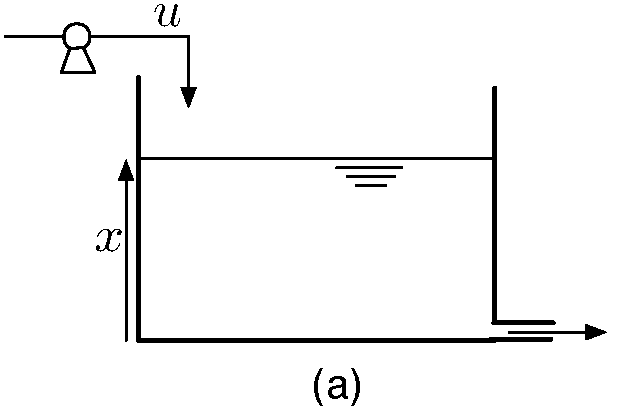
\includegraphics[width=6cm]{reseecouli}
%\end{center} \end{figure}
%\begin{figure}[ht] 
%\begin{center}
\hspace{1cm}
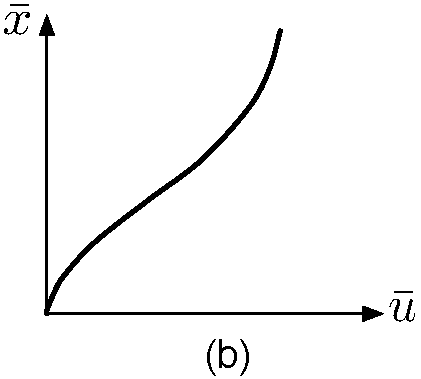
\includegraphics[width=4cm]{diagecouli}
\caption{(a) Réservoir à écoulement libre (b) Diagramme d'\'equilibre}
\label{fig:diagecouli}
\end{center} 
\end{figure}

Le  mod\`ele d'\'etat de ce syst\`eme a \'et\'e \'etabli au chapitre 4~:
\eqnn
\dot x = - \frac {kx\sqrt{x} }{S \beta + x} +u,
\eeqnn
o\`u $x$ repr\'esente le volume du liquide contenu dans le r\'eservoir.
Les \'equilibres du syst\`eme v\'erifient la relation $k \bar x \sqrt{\bar
x} = \bar u (S \beta + \bar x)$ dont le graphe dans $\real^2$ porte le nom de {\em
diagramme d'\'equilibre} (Fig. \ref{fig:diagecouli}).
On observe sur ce graphe qu'il y a un \'etat d'\'equilibre $\bar x$
distinct pour chaque valeur distincte de $\bar u \geq 0$ et que tous les
\'equilibres sont isol\'es. \qed
\end{exemple}
\vv

\begin{exemple}{\bf{\em R\'eservoir \`a \'ecoulement forc\'e}}

Consid\'erons maintenant le m\^eme r\'eservoir que pr\'ec\'edemment 
mais en supposant que l'\'ecoulement est forc\'e par une pompe dont le
d\'ebit volum\'etrique $F_0$ est constant (Fig. \ref{fig:diagecoufor}).
\begin{figure}[ht]
\begin{center}
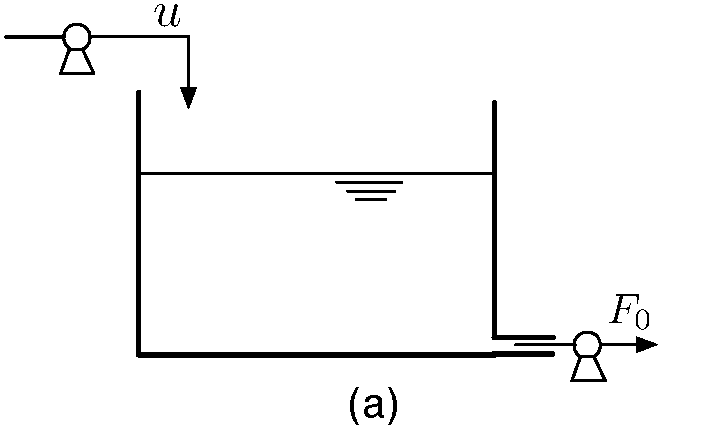
\includegraphics[width=6.5cm]{resecoufor}
\hspace{1cm}
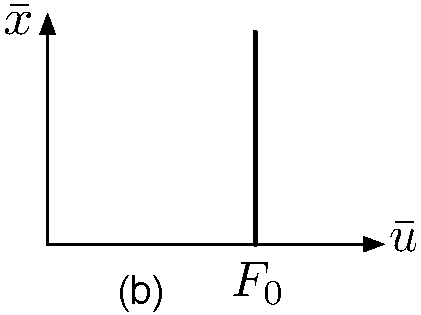
\includegraphics[width=40mm]{diagecoufor}
\caption{(a) Réservoir à écoulement forcé. (b) Diagramme d'\'equilibres.}
\label{fig:diagecoufor}
\end{center} 
\end{figure}
Le mod\`ele
d'\'etat devient alors~:
$$\dot x=-F_0 + u.$$
Comme dans l'exemple pr\'ec\'edent, le syst\`eme est \`a
l'\'equilibre lorsque le d\'ebit d'entr\'ee compense exactement le
d\'ebit de sortie~:
$$\bar u=F_0.$$
Cette fois, il n'y a qu'une seule valeur possible de l'entr\'ee $u$
qui donne lieu \`a un \'equilibre. Par contre, l'\'etat d'\'equilibre
$\bar x$ peut prendre n'importe quelle valeur positive. Le diagramme
d'\'equilibre est illustr\'e \`a la figure \ref{fig:diagecoufor}. On observe
que les
\'equilibres ne sont pas isol\'es puisque $\bar x$ est
ind\'etermin\'e. \qed
\end{exemple}
\vv

\begin{exemple}{\bf{\em Cuve de m\'elange \`a volume constant}}

Consid\'erons une cuve de m\'elange de volume $V$ constant et
parfaitement m\'elang\'ee (Fig.\ref{fig:diagcuvmel}(a)). 
\begin{figure}[ht] 
\begin{center}
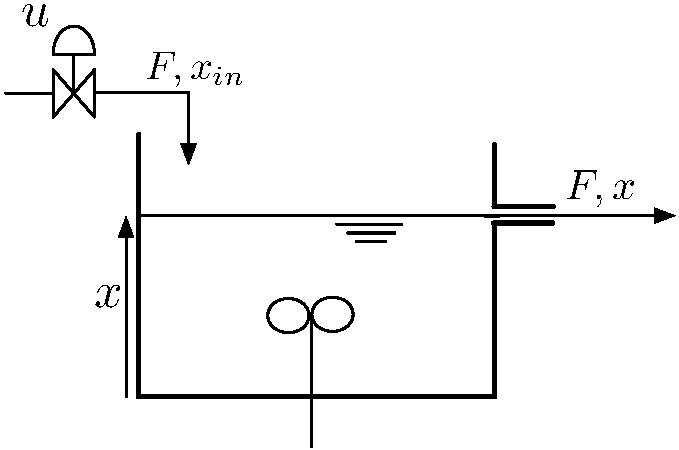
\includegraphics[width=60mm]{cuvmelvolcon}
\hspace{1cm}
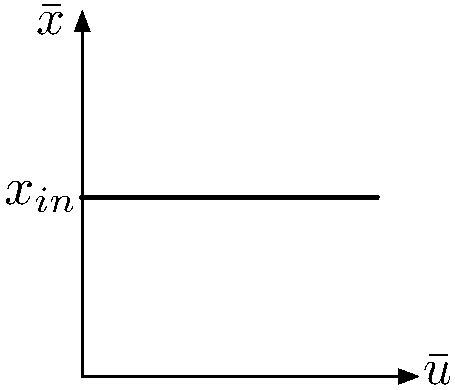
\includegraphics[width=35mm]{diagcuvmel}
\caption{(a) Cuve de m\'elange \`a volume constant. (b) Diagramme d'équilibres.}
\label{fig:diagcuvmel}
\end{center} 
\end{figure}
Le d\'ebit d'alimentation
transporte une substance en solution (par exemple un colorant) de
concentration $x_{in}$. Le d\'ebit d'alimentation $F$ est contrôl\'e
par une vanne de caract\'eristique~:
$$F=k u+b\;\;\;k>0,\;\;b>0,$$
o\`u $u$ d\'esigne l'ouverture de la vanne.

L'\'etat du syst\`eme est la concentration $x$  en colorant dans la
cuve et le mod\`ele d'\'etat s'\'ecrit~:
$$\dot x= (x_{in}-x)\frac{k u+b}{V}.$$

Le syst\`eme est \`a l'\'equilibre lorsque le d\'ebit massique de
colorant \`a l'entr\'ee compense exactement le d\'ebit massique \`a
la sortie~:
$$\frac{k \bar u +b}{V}x_{in}=\frac{k \bar u +b}{V}\bar x,$$
ce qui implique $\bar x =x_{in}$.
Le diagramme d'\'equilibre illustr\'e \`a la figure \ref{fig:diagcuvmel}(b) montre que
l'\'etat d'\'equilibre est fix\'e et isol\'e mais que l'entr\'ee
constante correspondant \`a cet \'etat d'\'equilibre est
ind\'etermin\'ee. \qed
\end{exemple}
\vv

\begin{exemple}{\bf{\em Cuve de m\'elange \`a \'ecoulement forc\'e}}

Jusqu'\`a pr\'esent, nous avons consid\'er\'e des exemples où le vecteur d'\'etat est de
dimension 1. Dans les syst\`emes de dimension sup\'erieure, les
diverses configurations d\'ecrites plus haut peuvent coexister, comme nous l'illustrons
maintenant en prenant comme exemple une cuve de m\'elange \`a
\'ecoulement forc\'e (Fig. \ref{fig:cuvecoufor}).
\begin{figure}[ht]
\begin{center}
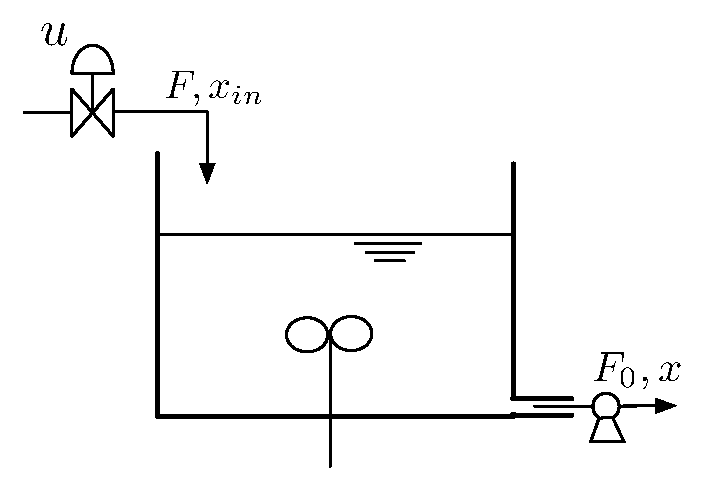
\includegraphics[width=7cm]{cuvecoufor}
\caption{Cuve de m\'elange \`a \'ecoulement forc\'e}
\label{fig:cuvecoufor}
\end{center} 
\end{figure}
Le mod\`ele d'\'etat de ce
syst\`eme, en notant $x_1$ le volume de la cuve et $x_2$
la concentration en colorant dans celle-ci, s'\'ecrit~:
\begin{equation*} \begin{split}
\dot x_1&= -F_0+k u+b,\\
\dot x_2&=(x_{in}-x_2)\frac{k u+b}{x_1}.
\end{split} \end{equation*}
Dans ce cas ci, le diagramme d'\'equilibre se repr\'esente en dimension 
3 (Fig.~\ref{fig:diagcuvemelcoufor}) et on constate qu'il y a une seule valeur de l'entr\'ee
qui donne lieu \`a un \'equilibre, $\bar u=(F_0-b)/k$, et que pour
cette valeur $\bar u$, le volume d'\'equilibre $\bar x_1$ est
ind\'etermin\'e alors que la concentration \`a l'\'equilibre vaut
$\bar x_2=x_{in}$. \qed
\begin{figure}[h]
\begin{center}
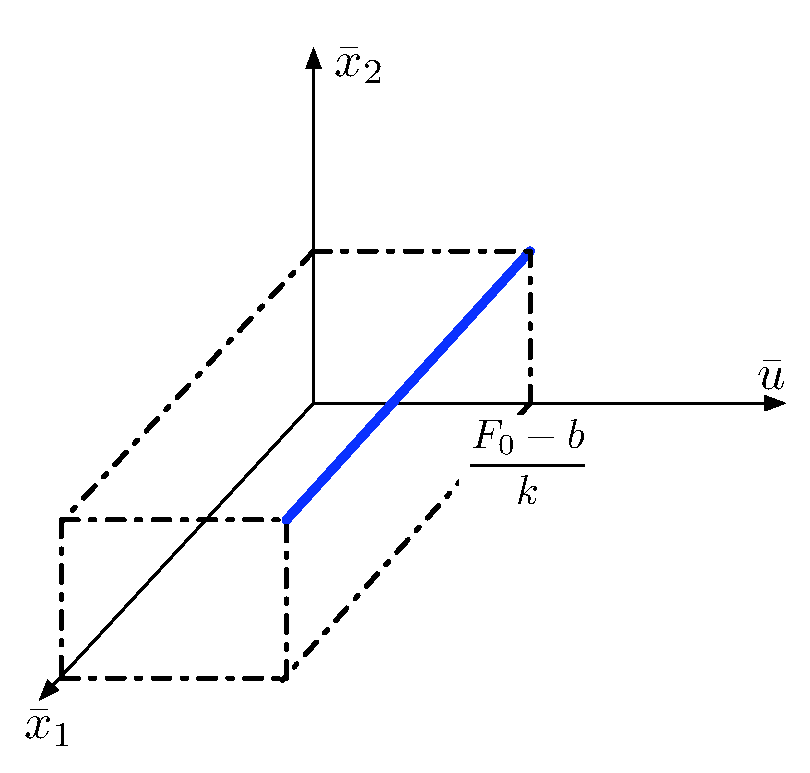
\includegraphics[width=6cm]{diagcuvemelcoufor}
\caption{Diagramme d'\'equilibre pour la cuve de m\'elange \`a
\'ecoulement forc\'e}
\label{fig:diagcuvemelcoufor}
\end{center} 
\end{figure}
\end{exemple}

Les exemples de dimension 1 ou 2 consid\'er\'es jusqu'\`a pr\'esent
ont illustr\'e des situations o\`u
\begin{itemize}
\item soit le syst\`eme poss\`ede un \'equilibre isol\'e pour
chaque valeur de l'entr\'ee $\bar u$,
\item soit le syst\`eme poss\`ede une infinit\'e d'\'equilibres
non isol\'es correspondant \`a une valeur pr\'ecise de $\bar u$.
\end{itemize}
Pour les syst\`emes non-lin\'eaires, d'autres configurations
sont possibles. En particulier, on peut observer plusieurs
\'equilibres isol\'es correspondant \`a une m\^eme valeur de $\bar u$ comme
cela est illustr\'e dans l'exemple suivant.

\begin{exemple}{\bf{\em R\'eacteur chimique}}

Consid\'erons un r\'eacteur chimique continu parfaitement m\'elang\'e dans lequel se produit une
r\'eaction exothermique irr\'eversible $A \longrightarrow B$. Le mod\`ele d'\'etat s'\'ecrit comme suit (voir Chapitres 1 et 5)~:
\begin{equation*} \begin{split} 
\dot x_A &= -kx_A e^{-\frac{\alpha}{T}}+D(x_A^{in}-x_{A}),\\
\dot x_{B} &= kx_{A} e^{-\frac{\alpha}{T}}-D x_{B},\\
\dot T &= hkx_{A} e^{-\frac{\alpha}{T}}-qT+u,
\end{split} \end{equation*}
où $x_{A}$ et $x_{A}^{in}$ sont les concentrations en r\'eactif $A$
dans le r\'eacteur et dans l'alimentation, $x_B$ est la concentration en produit $B$, $D$ est le d\'ebit volum\'etrique suppos\'e constant d'alimentation et de sous-tirage,
$T$ est la temp\'erature et $u$ est l'apport calorifique par unit\'e
de temps.

Les \'equilibres de ce syst\`eme sont caract\'eris\'es par les
\'equations
\begin{equation*} \begin{split}
\bar x_{A}&=\frac{Dx_{A}^{in}}{k e^{-\alpha/\bar T}+D}, \\
\bar x_{B}&=\frac{k \bar x_{A} e^{-\alpha/\bar T}}{D}, \\
\bar T&=\frac{1}{q}\left(\frac{Dx_{A}^{in}hk  e^{-\alpha/\bar T}}{k
 e^{-\alpha/\bar T}+D} + \bar u \right).
\end{split} \end{equation*}
La troisi\`eme \'equation permet de d\'eterminer $\bar T$ en fonction de $\bar u$. Les deux premi\`eres permettent alors de d\'eduire de $\bar T$ des valeurs d'\'equilibre pour $\bar x_{A}$ et $\bar x_{B}$. 
\begin{figure}[h]
\begin{center}
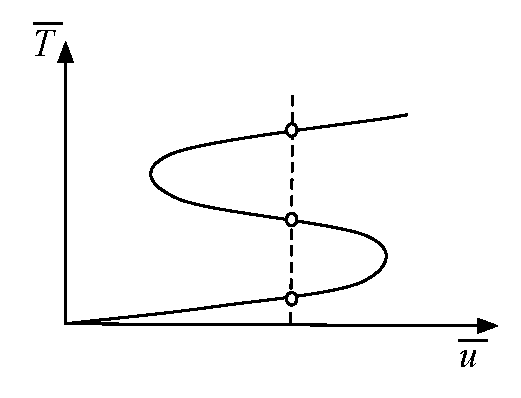
\includegraphics[height=4.4cm]{eqS}
\caption{Diagramme d'\'equilibre pour un r\'eacteur chimique simple}
\label{fig:eqS}
\end{center} 
\vspace{-5mm}
\end{figure}
Le diagramme d'\'equilibre repr\'esentant $\bar T$ en fonction de $\bar u$ est
illustr\'e \`a la figure \ref{fig:eqS}.
Suivant les valeurs de $\bar u$, on constate donc qu'il
existe un, deux ou trois
\'equilibres isol\'es.\qed
\end{exemple}

\section{\'Equilibres des syst\`emes lin\'eaires} 

Soit le syst\`eme lin\'eaire 
\eqnn
\dot x = Ax + Bu \label{syslin}
\eeqnn
pour lequel l'\'equation d\'efinissant
les \'equilibres devient
\eqnn A \bar x + B \bar u = 0. \eeqnn
Les \'equilibres d'un syst\`eme lin\'eaire sont compl\`etement
caract\'eris\'es par le th\'eor\`eme suivant.

\begin{theoreme}{\blanc}
\begin{itemize}
\item  Si la matrice $A$ est r\'eguli\`ere, alors pour tout $\bar u$, le couple
$(-A^{-1}B\bar u,\bar u)$ est un \'equilibre isol\'e.
\item Si la matrice $A$ est singuli\`ere, le syst\`eme
(\ref{syslin}) a une infinit\'e d'\'equilibres (non isol\'es) pour
autant que $B\bar u \in \mbox{Im}A$. Ces \'equilibres sont la
vari\'et\'e affine solution du syst\`eme $A \bar x = -B \bar u$. Par
contre, pour tout $\bar u$ tel que $B\bar u \notin \mbox{Im}A$, le
syst\`eme (\ref{syslin}) ne poss\`ede pas d'\'equilibre. \qed
\end{itemize}
\end{theoreme}

Pour les syst\`emes dynamiques lin\'eaires, on ne peut donc pas avoir
plusieurs
\'equilibres isol\'es correspondant \`a la m\^eme valeur de l'entr\'ee
$\bar u$.  Remarquons enfin que le couple $(\bar x, \bar u) = (0,0)$ est toujours un
\'equilibre pour un syst\`eme dynamique lin\'eaire de la forme (\ref{syslin}).

\begin{exemple}{\bf{\em Mod\`eles lin\'eaires de machines DC}}

Plusieurs mod\`eles de machines \`a courant continu (moteurs et
g\'en\'eratrices) ont \'et\'e pr\'esent\'es \`a la section~3.6. Sous
les hypoth\`eses g\'en\'erales de frottement visqueux lin\'eaire et
de non-saturation des flux, certains de ces mod\`eles sont
lin\'eaires. Nous examinons ci-dessous leur configuration
d'\'equilibre.\\

\noindent{\em G\'en\'eratrice DC command\'ee par le stator}

On consid\`ere le mod\`ele d'\'etat d'une g\'en\'eratrice \`a courant continu tournant \`a {\it vitesse $\omega$ constante}. En notant $x_1=I_s$, le courant statorique, $x_2=I_r$, le courant rotorique et $u=v_s$ la tension aux bornes du circuit statorique, le mod\`ele d'\'etat est lin\'eaire et s'\'ecrit comme suit~:
$$
\bma{c}\dot x_1\\ \dot x_2
\ema=\bma{ccc}-\dfrac{R_s}{L_s} & & 0\\ & \vspace{-2mm} & \\ K_e\omega & &-\dfrac{R_r+R_L}{L_r}\ema
\bma{c}x_1\\x_2 \ema + \bma{c} \dfrac{1}{L_{s}}\\ \vspace{-2mm} \\ 0\ema u
$$
La matrice $A$ de ce syst\`eme lin\'eaire est inversible et la
g\'en\'eratrice poss\`ede donc un \'etat d'\'equilibre isol\'e pour
chaque valeur de la tension d'entr\'ee $\bar u$~:
\eqnn
\bar x_1&=&\dfrac{L_s}{R_s}\bar u\\
\bar x_2&=&\dfrac{L_r}{R_r+R_L}\dfrac{L_s}{R_s}K_e\omega \bar u
\eeqnn

\noindent{\em Moteur DC command\'e par le rotor}

Avec comme variables d'\'etat pour ce syst\`eme
$x_1=\theta$, la position angulaire du rotor, $x_2=\dot \theta=\omega$, la vitesse de rotation et $x_3=I_r$, le courant rotorique, on obtient le
mod\`ele suivant~:
$$\bma{c}\dot x_1\\ \dot x_2\\ \dot x_3\ema =
\bma{ccc}0&1&0\\ $ \vspace{-2mm} $ \\ 0&-\dfrac{B}{J}&\dfrac{K_mI_s}{J}\\ $ \vspace{-2mm} $ \\
0&-\dfrac{K_e I_s}{L_r} &-\dfrac{R_r}{L_r}\ema \bma{c}x_1\\x_2\\x_3\ema
+\bma{cc}0&0\\ &\vspace{-2mm} \\ 0&\dfrac{1}{J}\\ &\vspace{-2mm} \\ \dfrac{1}{L_r}& 0\ema \bma{c}u_1\\u_2\ema
$$
o\`u $u_1$ est le couple r\'esistant et
$u_2$ la tension de commande de l'induit.
On observe que :
\begin{itemize}
\item la matrice d'\'etat $A$ du syst\`eme est singuli\`ere,
\item $B\bar u =(0\;\; \bar u_2/J\;\;\bar u_1/L_r)^T \notin \mbox{Im} A$
sauf si $\bar u_1/\bar u_2=-R_r/K_mI_s$ ou si $\bar u_1=\bar u_2=0$.
\end{itemize}
Le premier cas correspond \`a une tension de commande rotorique qui cr\'ee un couple moteur compensant exactement le couple r\'esistant. La vitesse de rotation est alors nulle et la position angulaire du rotor est ind\'etermin\'ee. La valeur d'\'equilibre du courant rotorique est donn\'ee par $\bar x_3=\bar I_r=\bar u_2/K_m I_s$.
Dans le deuxi\`eme cas, les \'equilibres sont  de la forme $\bar x_1=\bar \theta, \bar
x_2=0, \bar x_3=0$, c.\`a.d. que le moteur est \`a l'arr\^et avec
le rotor dans une position angulaire quelconque.

On peut  examiner aussi les \'equilibres du
sous-syst\`eme dont les \'etats sont la vitesse $\omega$ et le
courant $I_r$~:
$$\bma{c} \dot x_2\\ \dot x_3\ema =
\bma{cc}-\dfrac{B}{J}&\dfrac{K_m I_s}{J}\\ & \vspace{-2mm} \\
-\dfrac{K_e I_s}{L_r} &-\dfrac{R_r}{L_r}\ema \bma{c}x_2\\x_3\ema
+\bma{cc}0&\dfrac{1}{J}\\ & \vspace{-2mm} \\ \dfrac{1}{L_r}& 0\ema \bma{c}u_1\\u_2\ema.
$$ 
La matrice d'\'etat de ce syst\`eme est
inversible (toutes les constantes sont positives et le d\'eterminant ne s'annule donc pas) et \`a chaque valeur du vecteur d'entr\'ee $\bar u$
correspondra une valeur d'\'equilibre du vecteur d'\'etat $(\bar
x_1\;\;\bar x_2)^T$. Cette situation d'\'equilibre, qui n'est en rien
contradictoire avec la pr\'ec\'edente, correspond au cas d'un moteur DC qui
entra\^{\i}ne une charge en tournant \`a vitesse constante. \qed
\end{exemple}

\section{Invariants}

La notion d'invariant que nous allons d\'efinir dans cette section est une
g\'en\'eralisation de la notion d'\'equilibre.

\begin{definition}{\bf{\em Invariant}}

Le sous-ensemble $\mathcal{X} \times U \subset \real^n \times \real^m$ est un invariant
du syst\`eme dynamique $\dot x = f(x,u)$ si :
\eqnn
\left\{
\begin{array}{l}
x(t_0) \in \mathcal{X}\\
u(t) \in U \;\;\;\forall t \geq t_0 
\end{array}\right\} & \Rightarrow & \left\{\begin{array}{l} 
x(t) \text{ existe}\\ x(t) \in \mathcal{X} \end{array} \right\}\forall t \geq t_0 \xqedhere{2cm}{\qed} 
\eeqnn
\end{definition}

Cette d\'efinition signifie donc que si l'\'etat du syst\`eme se trouve dans $\mathcal{X}$ \`a
un instant initial, il y restera \`a tous les instants ult\'erieurs tant que le
signal d'entr\'ee $u(t)$ sera lui-même maintenu dans $U$.

Nous avons d\'ej\`a rencontr\'e plusieurs exemples d'invariants dans les chapitres
pr\'ec\'edents.  L'exemple le plus simple est l'ensemble des \'equilibres d'un
syst\`eme correspondant \`a une entr\'ee $\bar u$ constante.  Dans ce cas, le
sous-ensemble $U = \{\bar u\}$  est r\'eduit \`a un singleton tandis que $\mathcal{X}$
contient le ou les \'etats d'\'equilibres $\bar x$ correspondants.  

Un autre exemple typique est l'{\em orthant positif} $(\mathcal{X} = \real^n_+) \times (U \subset \real^m)$ 
qui est, par d\'efinition, un invariant pour les syst\`emes positifs
(voir D\'efinition 4.3 et Th\'eor\`eme 4.4.).

Il y a diverses mani\`eres de caract\'eriser les invariants d'un syst\`eme
dynamique selon la forme particuli\`ere que prend le sous-ensemble $\mathcal{X}$.  Nous
allons pr\'esenter deux caract\'erisations remarquables : dans la premi\`ere $\mathcal{X}$
est un ouvert de $\real^n$, dans la seconde $\mathcal{X}$ est une
hypersurface dans $\real^n$.  \\

\noindent{\bf $\bullet$ \!$\mathcal{X}$  est un ouvert dans $\real^n$}

Soit $\mathcal{X}$ un sous-ensemble ouvert de  $\real^n$ dont la fronti\`ere $\partial \mathcal{X}$ est suffisamment régulière.  Si en tout
point $y$ de la fronti\`ere $\partial \mathcal{X}$, le vecteur $f(y,v)$ pointe vers
l'int\'erieur de $\mathcal{X}$ pour tout $v \in U$, alors le sous-ensemble $\mathcal{X} \times U$
est un invariant du syst\`eme $\dot x = f(x,u)$.

Cette caract\'erisation d'un invariant sera illustr\'ee au chapitre 8 (section 8.4).\\

\noindent{\bf $\bullet$ \!$\mathcal{X}$ est une hypersurface de niveau dans $\real^n$}

On appelle {\it int\'egrale premi\`ere} une fonction $z = h(x)$ de classe $C^2$ telle que~:
\eqn
\frac {\partial h}{\partial x}f(x,u) = 0 \;\;\; \forall u \in U. \label{condit}
\eeqn
On d\'efinit le sous-ensemble $\mathcal{X}$ comme suit :
\eqnn
\mathcal{X} \triangleq \{x \in R^n : h(x) = c \}
\eeqnn
avec $c$ constante r\'eelle quelconque.
Cet ensemble $\mathcal{X}$ est une hypersurface dans $\real^n$.  Comme la condition (\ref{condit}) implique que la fonction $z = h(x)$ est constante le long des trajectoires, il est \'evident que le sous-ensemble
$\mathcal{X} \times U$ est un invariant du syst\`eme $\dot x = f(x,u)$.  Les
{\em invariants r\'eactionnels} en constituent une illustration typique. 

\begin{exemple}{\bf{\em Les invariants r\'eactionnels}}

Ainsi que nous l'avons vu au chapitre 5, le mod\`ele d'\'etat d'un r\'eacteur continu parfaitement m\'elang\'e s'\'ecrit comme suit~:
\eqn
\dot x = Cr(x) + u(x^{in} -x) \label{reacteur}
\eeqn
où $x$ est la composition du milieu r\'eactionnel, $u$ le d\'ebit d'alimentation,
$x^{in}$ la composition (suppos\'ee constante) de l'alimentation, $C$ est la
matrice stoechiom\'etrique et $r(x)$ est le vecteur des cin\'etiques de r\'eaction.

Le d\'ebit $u$ est positif et born\'e par la capacit\'e maximale de la pompe
d'alimentation $u_{\max}$, de sorte que nous d\'efinissons $U$ comme l'intervalle
ferm\'e :
\eqnn
U = [0, u_{\max}]
\eeqnn
D'autre part, le sous-ensemble $\mathcal{X}$ est d\'efini comme suit :
\eqnn
\mathcal{X} =\{x:x\in \real^n_+, \;\; Lx = Lx^{in}\}
\eeqnn
où $L$ est une matrice $(n-p)\times n$ telle que $LC=0$.  En d'autres termes,
les lignes de $L$ forment une base du noyau de la transpos\'ee de la matrice 
stoechiom\'etrique
$C$.

Le sous-ensemble $\mathcal{X} \times U$ ainsi d\'efini constitue un invariant du syst\`eme
(\ref{reacteur}).  Pour le v\'erifier, nous consid\'erons la transformation
lin\'eaire partielle d'\'etat :
\eqnn
z = Lx
\eeqnn
dont nous calculons l'\'evolution le long des trajectoires du syst\`eme :
\eqnn
\dot z = LCr(x) + u(Lx^{in} -Lx) =   u(Lx^{in} -Lx) \;\; \mbox{car } LC=0
\eeqnn
Selon la d\'efinition de $\mathcal{X}$, on observe imm\'ediatement que, si $Lx(t_0) =
Lx^{in}$, alors $\dot z =0$ le long des trajectoires du syst\`eme et donc
$Lx(t)= Lx^{in} \;\;\;\forall t \geq t_0$, et ceci ind\'ependamment du signal
d'entr\'ee $u(t)$.

D'autre part, le syst\`eme (\ref{reacteur}) est un syst\`eme positif et donc
$x(t) \in \real^n_+$ $\forall t \geq t_0$ si $x(t_0) \in \real^n_+$ et si $u(t) \in U
\;\forall t \geq t_0$.

Les invariants d\'efinis de cette mani\`ere portent le nom d'invariants
r\'eactionnels ou encore d'invariants chimiques dans la litt\'erature. \qed
\end{exemple}


\section{Exercices}

\begin{exercice}{\bf \em Un relais électromagnétique}

D\'eterminer les \'equilibres du mod\`ele d'\'etat d'un relais \'electromagn\'etique donn\'e au chapitre 3, exemple 3.2 (voir aussi l'exercice 6.2). \qed
\end{exercice}
\vv

\begin{exercice}{\bf \em G\'en\'eratrice \`a courant continu}

On consid\`ere le mod\`ele d'une g\'en\'eratrice \`a courant continu (voir chapitre 3, section 3.6) d\'ebitant sur une charge r\'esistive avec un frottement visqueux lin\'eaire.
\begin{enumerate}
\item Calculer les \'equilibres en fonction des entr\'ees $\bar u_1$ et $\bar u_2$
\item D\'eterminer les points de fonctionnement optimaux qui maximisent le courant d\'ebit\'e par la g\'en\'eratrice. \qed
\end{enumerate}
\end{exercice}
\vv

\begin{exercice}{\bf \em Une boucle à asservissement de phase}

Une boucle à asservissement de phase (phase-locked loop) utilisée dans les réseaux  de communication est décrite par l'équation
\eqnn
\ddot y + (a + b \cos y) \dot y + u \sin y = 0
\eeqnn
avec $a > b > 0$ et $u(t) > 0 \, \forall t$. 
\begin{enumerate}
\item Mettre le système sous forme d'un modèle d'état.
\item Déterminer les équilibres.
\end{enumerate}
\end{exercice}
\vv

\begin{exercice}{\bf \em Un bateau}

Déterminer les équilibres du modèle d'état du bateau de l'exercice 2.7. Quel est le sens physique de ces équilibres ? \qed
\end{exercice}
\vv 

\begin{exercice}{\bf \em Un broyeur industriel}

\begin{figure}[htbp] 
   \centering
   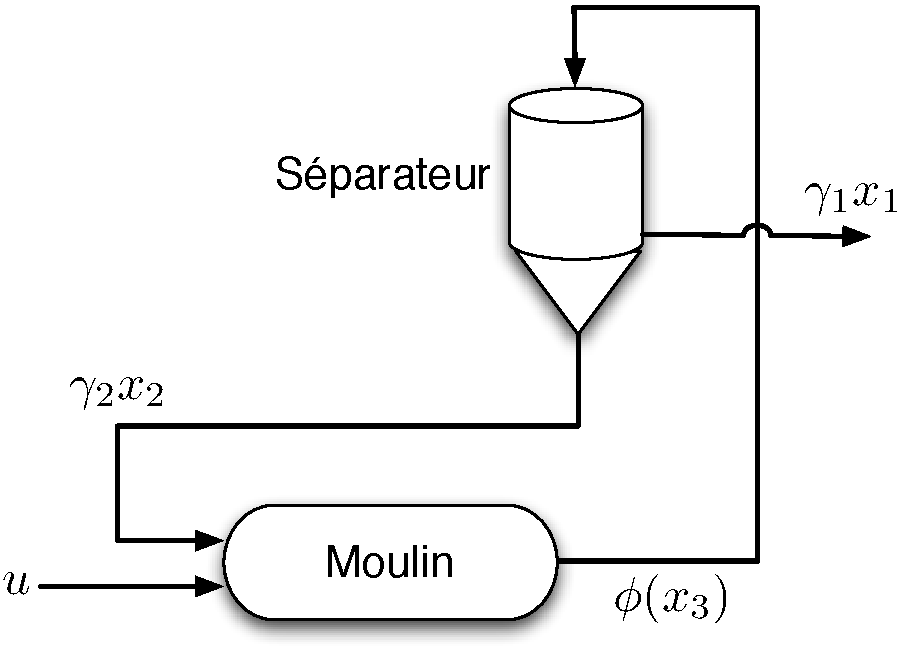
\includegraphics[height=5cm]{broyeur} \hfill
	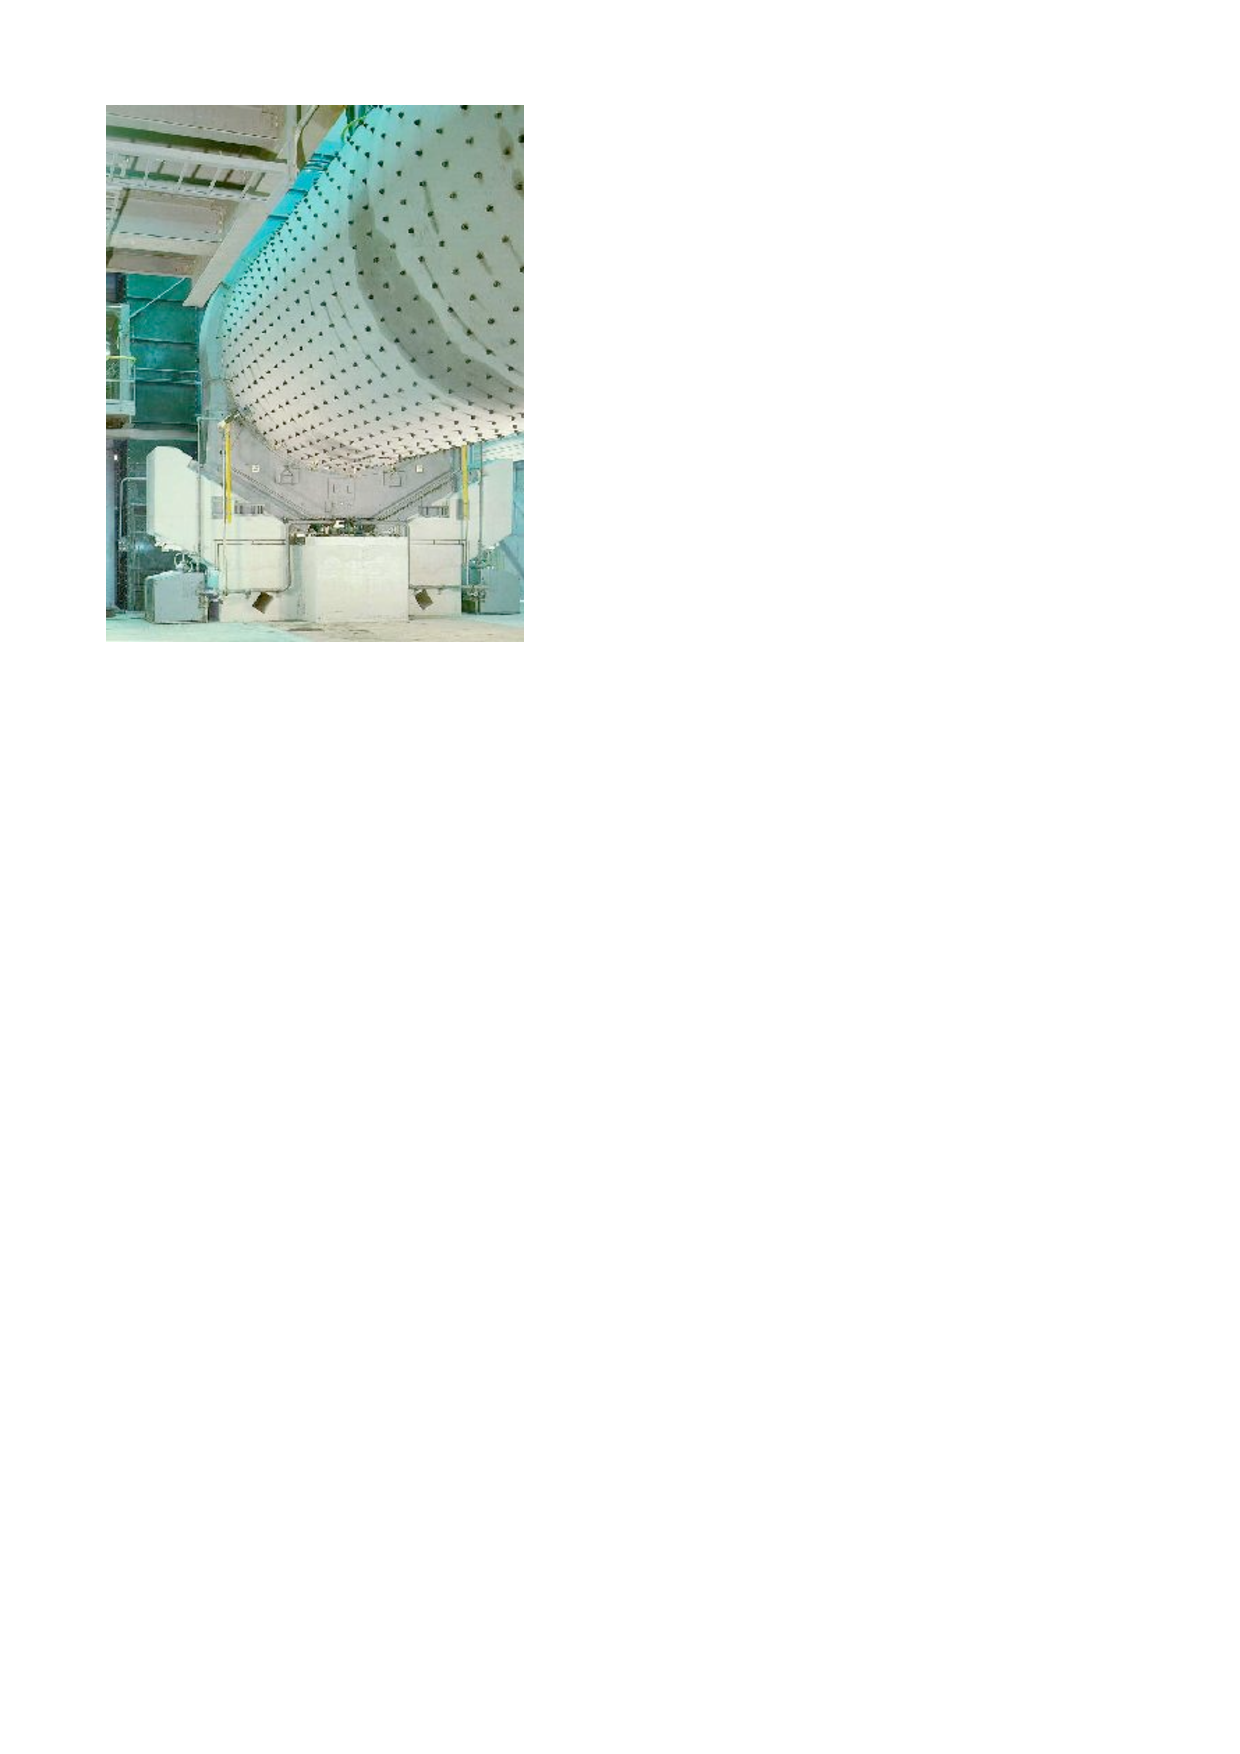
\includegraphics[height=5cm]{broyeur-photo}
   \caption{Circuit de broyage - Photo d'un broyeur industriel}
   \label{fig:broyeur}
\end{figure}
Le fonctionnement d'un circuit de broyage industriel (fig. \ref{fig:broyeur}) est d\'ecrit par le mod\`ele d'\'etat~:
\begin{equation*} \begin{split} 
\dot x_1 &= -\gamma_1 x_1 +(1-\alpha) \phi(x_3),\\
\dot x_2 &= -\gamma_2 x_2 +\alpha \phi(x_3),\\
\dot x_3 &= \gamma_2 x_2 - \phi(x_3)+u.
\end{split} \end{equation*}
avec les notations suivantes~:\\

\begin{tabular}{ll}
$x_1$&= quantit\'e de produit fini dans le s\'eparateur;\\
$x_2$&= quantit\'e de mati\`ere recycl\'ee dans le s\'eparateur;\\
$x_3$&= quantit\'e de mati\`ere dans le broyeur:\\
$u $&= d\'ebit d'alimentation du broyeur.
\end{tabular}\\

\noindent Le param\`etre $\alpha$ est la constante caract\'eristique du s\'eparateur. 
($0 < \alpha < 1$). La fonction de broyage $\phi(x_3)$ est de la forme suivante~:
\eqnn
\phi(x_3) = k_1x_3e^{-k_2x_3}
\eeqnn
où $k_1$ et $k_2$ sont des constantes positives.
\begin{enumerate}
\item Montrer qu'il s'agit d'un syst\`eme \`a compartiments et donner le graphe du syst\`eme.
\item D\'eterminer les \'equilibres du syst\`eme.
\item L'ensemble d\'ecrit par les in\'egalit\'es suivantes caract\'erise une situation de bourrage de l'installation. Montrer qu'il s'agit d'un invariant du syst\`eme.
\begin{equation*} \begin{split} 
&  x_1 \geq 0, \hspace{5mm} x_2 \geq 0, \hspace{5mm} x_3 \geq 0, \\
&  (1 - \alpha)\phi(x_3) \leq \gamma_1x_1 < \bar u, \\ 
&  \alpha \phi(x_3) \leq \gamma_2x_2, \\ 
&  \frac{\partial\phi(x_3)}{\partial x_3} < 0. \xqedhere{6.5cm}{\qed}
\end{split} \end{equation*}
\end{enumerate}
\end{exercice}
\vv

\begin{exercice}{\bf \em Un r\'eacteur biochimique}

On consid\`ere le mod\`ele d'\'etat d'un r\'eacteur biochimique de l'exercice 6.2.
\begin{enumerate}
\item D\'eterminer les \'equilibres du syst\`eme et esquisser les diagrammes
d'\'equilibre.
\item D\'eterminer les invariants r\'eactionnels du syst\`eme.
\item Mêmes questions si la r\'eaction est r\'eversible. \qed
\end{enumerate}
\end{exercice}
\vv

\begin{exercice}{Dynamique d'une infection virale}

La dynamique d'un infection virale avec actions lytique et non-lytique d'immunisation est décrite par le modèle d'état suivant:
\begin{equation*} \begin{split}
\dot x_1 &= \lambda - dx_1 - \dfrac{\beta x_1 x_2}{1 + q x_3}, \\
\dot x_2 &= \dfrac{\beta x_1 x_2}{1 + q x_3} - a x_2 - p x_2 x_3, \\
\dot x_3 &= c x_2 - b x_3.
\end{split} \end{equation*}
Dans ces équations, $x_1$, $x_2$ et $x_3$ sont respectivement les quantités de cellules saines, infectées et immunes. Les cellules infectées produisent les particules virales. $\lambda$ est le taux de production des cellules saines et $d$ leur taux de mortalité. Les composants lytiques de l'activité anti-virale tuent les cellules infectées tandis que les composants non-lytique inhibent la réplication des particules virales. Les cellules infectées sont tuées  à la vitesse $p x_3$ où $p$ représente l'intensité de l'activité anti-virale lytique. La production des cellules infectées est représentée par le terme
$$
\dfrac{\beta x_1 x_2}{1 + q x_3}
$$
où $q x_3$ représente l'intensité d'inhibition de la réplication par l'activité antivirale non-lytique. Le taux de mortalité des cellules infectées est $a$ et le taux de mortalité des cellules immunes est $b$. Enfin $c x_2$ est le taux de production des cellules immunes.
\begin{enumerate}
\item Montrer que le modèle d'état est un système réactionnel.
\item Montrer que le modèle d'état est équivalent à un système à compartiments.
\item Déterminer les équilibres du système dans l'orthant positif.
\end{enumerate}
\end{exercice}
\vv


\begin{exercice}{\bf \em Syst\`eme m\'ecanique}

On consid\`ere le mod\`ele d'un syst\`eme m\'ecanique \`a un degr\'e de libert\'e~:
\eqnn
\ddot \theta + c \dot \theta + r \sin \theta = 0
\eeqnn
\begin{enumerate}
\item Ecrire le mod\`ele d'\'etat du syst\`eme ($x_1 = \theta$).
\item D\'eterminer les \'equilibres.
\item Montrer que, sous la condition $c^2 \geq 4 r$, existe un invariant born\'e (dont l'int\'erieur est non vide) dans l'orthant $\{ x_1 \geq 0, x_2 \leq 0 \}$. \qed
\end{enumerate}
\end{exercice}

\end{document}

